%!TEX program = xelatex
%%%%%%%%%%%%%%%%%%%%%%%这是导言部分的开始%%%%%%%%

%========= 导言部分声明文档的类型=================
\documentclass{article}

%=========导言部分可可以加载宏包=================
\usepackage{amsmath}                % 数学公式排版宏包
\usepackage{amssymb}                % 数学符号命令宏包
\usepackage{amsthm}                 % 数学定理宏包
\usepackage[UTF8]{ctex}             % 中文输入宏包
\usepackage[a4paper]{geometry}      % 页面设置宏包
\usepackage{setspace}               % 行间距宏包
\usepackage{graphicx}               % 图片宏包
\usepackage{listings}               % 代码宏包
\usepackage{color}					% 颜色宏包
\usepackage{xcolor}                 % 颜色处理宏包
\usepackage{float}                  % 浮动对象式样宏包
\usepackage{fontspec}
\usepackage{enumerate}				% 列举编号包

%=========页面设置==============================
\geometry{left=1cm,right=1cm,top=1cm,bottom=2cm}
\onehalfspacing
\setlength\parindent{0em}

%=========代码格式设置============================
\definecolor{dkgreen}{rgb}{0,0.6,0}
\definecolor{gray}{rgb}{0.5,0.5,0.5}
\definecolor{mauve}{rgb}{0.58,0,0.82}
% \setmonofont{Consolas}
\lstset{
	numbers = left, 	
	numberstyle = \color{gray}, 
	keywordstyle = \color{blue},
	commentstyle = \color{dkgreen}, 
	stringstyle = \color{mauve},
	basicstyle = \ttfamily,
	breaklines = true,
	frame = shadowbox, % 阴影效果
	rulesepcolor = \color{ red!20!green!20!blue!20} ,
	escapeinside = ``, % 英文分号中可写入中文
	xleftmargin = 2em,xrightmargin=2em, aboveskip=1em,
	framexleftmargin = 2em
} 

%=========导言部分可以定义标题信息===============
\title{组会报告}
\author{徐益}
\date{\today}
%%%%%%%%%%%%%%%%%%%%%%%这是导言部分的结束%%%%%%%%%

%%%%%%%%%%%%%%%%%%%%%%%这是正文部分的开始%%%%%%%%%
\begin{document}

%=========生成标题================================
\maketitle

%=========开始正文的输入==========================

%===========第一节=================
\section{工作内容} 
1. 完成matlab链路测试;

2. 实现系统发送端5G编码调制链路。

%===========第一节=================
\section{matlab链路测试结果}
\begin{figure}[H]
	\centering
	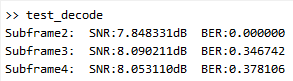
\includegraphics[width = .6\textwidth]{oldrst.png}
	\caption{原结果}
\end{figure}
\begin{figure}[H]
	\centering
	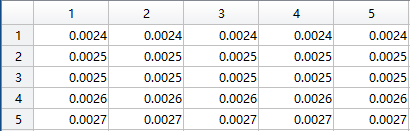
\includegraphics[width = .8\textwidth]{estn.png}
	\caption{估计噪声}
\end{figure}
\begin{figure}[H]
	\centering
	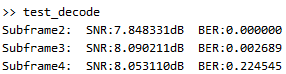
\includegraphics[width = .6\textwidth]{newrst.png}
	\caption{使用正确噪声后的结果}
\end{figure}

%===========第二节=================
\section{实现系统发送端5G编码调制链路}
\subsection{关于分流的系统改进}
\begin{figure}[H]
	\centering
	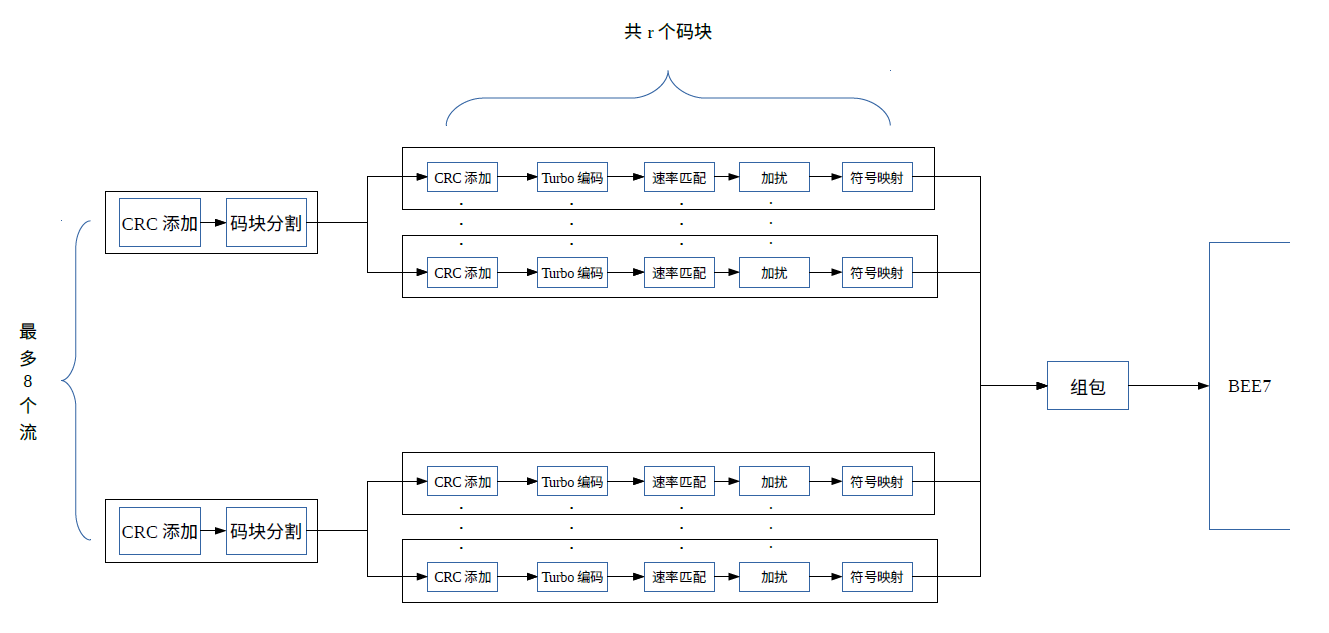
\includegraphics[width = \textwidth]{txstrulte.png}
	\caption{原系统}
\end{figure}
\begin{figure}[H]
	\centering
	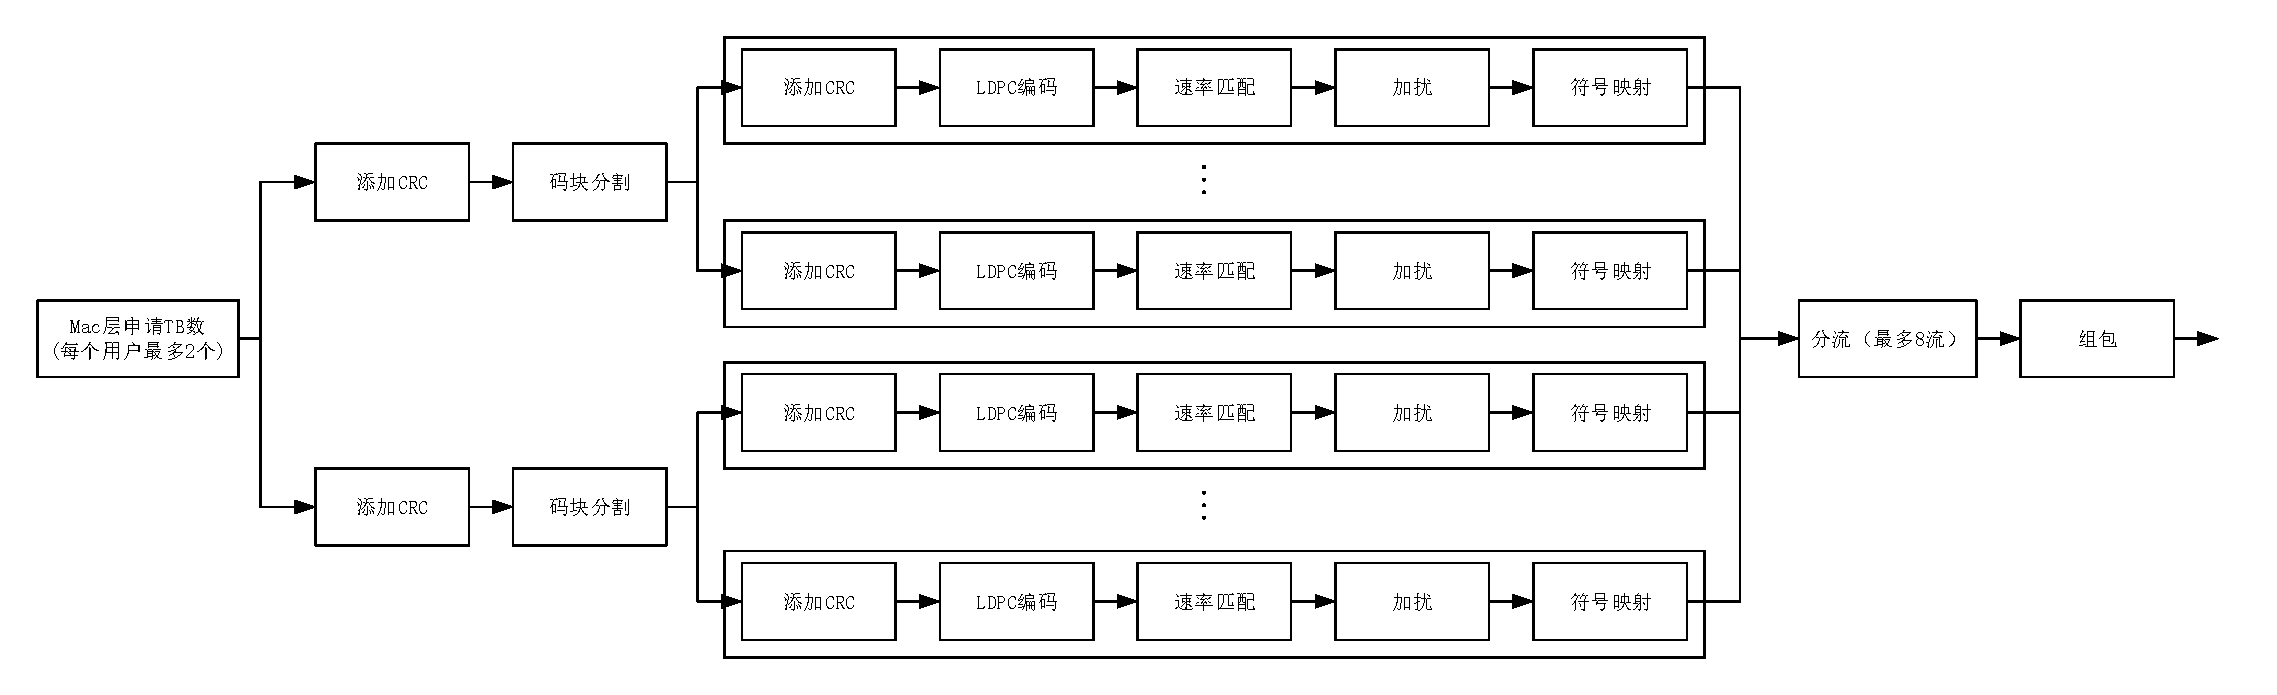
\includegraphics[width = \textwidth]{txstru5g.pdf}
	\caption{改进后系统}
\end{figure}
\subsection{关于初始化的代码修改}
\subsubsection{原LDPC部分代码结构}
\lstset{language=C++}
\begin{lstlisting}
…………
for(i = 0; i < LoopNum; i++)
{
	init_ldpc_param(ldpc_t, B, R);	// 初始化ldpc参数(包括空间分配)
	…………
	free_ldpc_t(ldpc_t);
}
…………
\end{lstlisting}
\subsubsection{先LDPC部分代码结构}
——对LDPC编译码空间分配与码长、码率解耦合
\lstset{language=C++}
\begin{lstlisting}
…………
init_ldpc_encoder_mem(ldpc_t);		// 编码相关空间分配(最大)
init_ldpc_decoder_mem(ldpc_t);		// 译码相关空间分配(最大)

for(i = 0; i < LoopNum; i++)
{
	init_ldpc_param(ldpc_t, B, R);	// 初始化ldpc参数(不包括空间分配)

	…………
}

free_ldpc_encoder_mem(ldpc_t);		// 编码相关空间释放
free_ldpc_decoder_mem(ldpc_t);		// 译码相关空间释放
…………
\end{lstlisting}

%===========第三节=================
% \section{根据PRACH测时延}
% \begin{figure}[H]
% 	\centering
% 	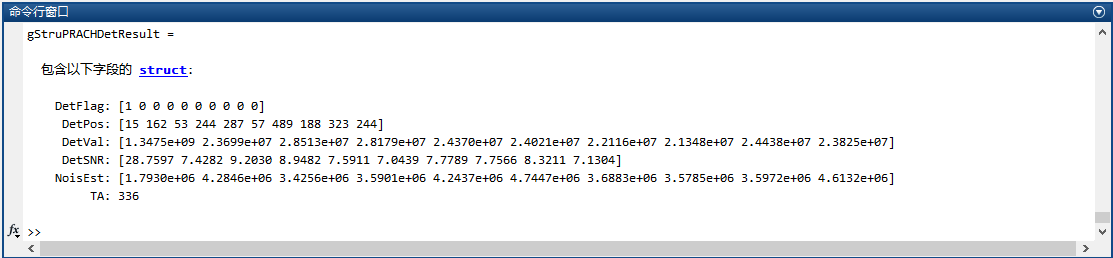
\includegraphics[width = \textwidth]{prach.png}
% 	\caption{时延测试结果}
% \end{figure}

%===========第四节=================
% \section{后续工作}
% 1. 实现当前SVN目录结构下基于LDPC的单线程编码调制链路;

%===========下周计划=================
\section{下阶段计划}
1. 实现接收端5G解调译码链路

\end{document}
%%%%%%%%%%%%%%%%%%%%%%%这是正文部分的结束%%%%%%%%%%%%